\sectionorchapter{Experimental asymptotics of
\texorpdfstring{$\CatalanNumber a\spc\of{a,b}$}{Ca spc(a,b)}}
Here we examine the exponential asymptotic behaviour of $\CatalanNumber a\spc\of{a,b}$ as a
function of $a+b$; this provides the asymptotics of the bound for
$\gn_{\pointset P}\of{\langle^a\rangle^b\langle^b\rangle^a}$. Specifically, we will be looking
at the behaviour for constant $\gh=\frac{b}{a}$.

The definition (\ref{spcDefinition}) of $\spc$,\begin{equation*}
\spc\of{a,b}\DefineAs
\sum{S\in\binom{[a]}{a-b}} \quad \prod{\gc\in\cells\of{[a] \setminus S}}\CatalanNumber {\Cardinality \gc}
\text,
\end{equation*}
has exponentially many terms in the sum for constant $\gh$, so it is highly impractical to compute.

However, using recurrence \ref{spcRecurrence1},
\begin{align*}\spc\of{a,b} &= \sum{i=0}[b]
\CatalanNumber {i}
\spc\of{a-i-1,b-i} &\text{for $b<a$,} \\
\spc\of{a,a} &= \CatalanNumber a \text,
\end{align*}
we can use memoization to compute $\spc\of{a,b}$ in cubic time.

We use the following \emph{Mathematica} code:
\begin{verbatim}
spc[a_, a_] := spc[a, a] = CatalanNumber[a];
spc[a_, b_] := spc[a, b] =
  Sum[spc[i, i] spc[a - i - 1, b - i], {i, 0, b}];
\end{verbatim}
Note that we replace the Catalan number $\CatalanNumber i$ in the summands by $\spc\of{i,i}$ in
order to benefit from the memoizatoin of Catalan numbers. While this doesn't visibly change the
order of the asymptotics for the values of $i$ that we are considering, it improves performance by
a noticeable constant.

This allows us to draw some plots (figure~\ref{figSpcExperimental}) to take an educated guess at
the behaviour of $\CatalanNumber a\spc\of{a,b}$. From this we can conjecture that
$\gn_{\pointset P}\of{\langle^a\rangle^b\langle^b\rangle^a}$ is at most $\BigO\of{5^n}$.

\begin{figure}[htb!]
\centering
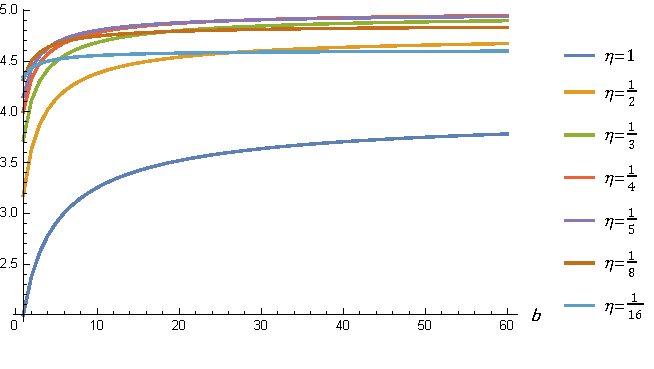
\includegraphics[scale=0.75]{spc-asymptotics}
\caption{Plots of $\pa{4^{a}\spc\of{a,b}}^{\frac{1}{a+b}}$,
where $a=\frac{b}{\gh}$,
as a fuction of $b$, for various values of $\gh$. As $b$ tends to infinity, this tends to the base
of the exponential bound.
We use $4^a$ rather than $\CatalanNumber a$ because we want to get rid of as many polynomial factors
as possible, since we are looking for the exponential behaviour.
Note that the topmost curve seems to asymptotically approach
$5$.\label{figSpcExperimental}}
\end{figure}